

\subsection{Downscale energy cascade of waves}
\label{subsection_cascade}



\begin{figure}
\centerline{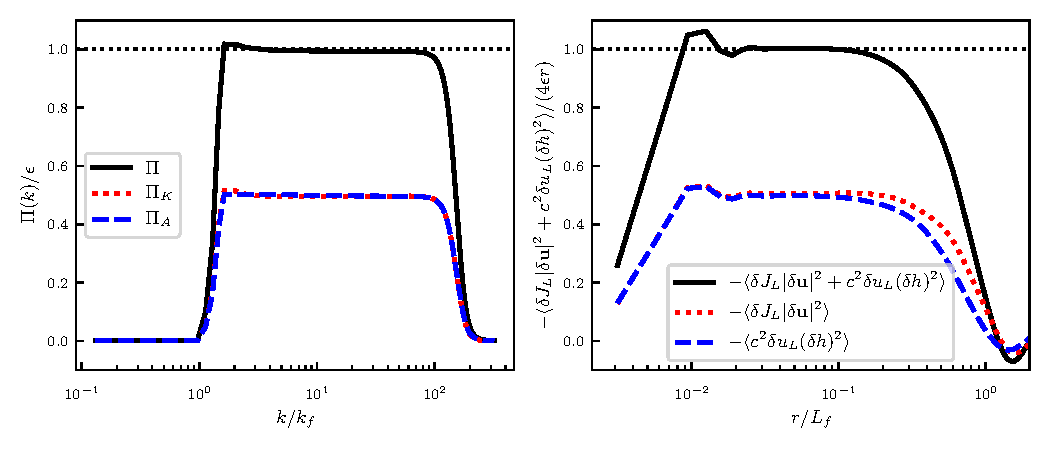
\includegraphics[width=\linewidth]{../Pyfig/fig_flux_struct_combined}}
\caption{(Left) Spectral energy fluxes averaged over a long simulation for $c
= 100$ and $n = 3840$.  The fluxes are nondimensionalized by $\eps$
and plotted versus $k/k_f$.
(Right)
Third order structure functions involved in the exact Kolmogorov law (\ref{eq_Kolmo})
averaged over a long simulation for $c = 20$ and $n = 3840$.
%
The structure functions are normalized by $4 \eps_q r$.
%
Black thick line, $\mean{ \delta J_L|\delta \uu|^2 }
+ c^2\mean{\delta u_L(\delta h)^2}$;
light thin line, $c^2\mean{\delta u_L (\delta h)^2}$;
dark thin line, $\mean{\delta J_L |\delta \uu|^2}$.
%
The dotted straight line shows $4 \eps_q r$,
where $\eps_q$ is the quadratic energy dissipation rate.
}
\label{fig_seb}
\end{figure}


The spectral energy fluxes of total energy, KE and APE are plotted in
figure~\ref{fig_seb} as functions of $k/k_f$.
%
The fluxes are approximately zero at the wave numbers smaller than the
forced wave numbers.  They increase sharply at the forced wave numbers
to values close to $\eps$ for the total energy flux and to $0.5\eps$
for the KE and APE fluxes.  The fluxes then decrease to zero over the
dissipation range.
%
The energy is transferred from the forced wave numbers to the
dissipation wave numbers with a constant flux equal to the mean
forcing and dissipation rates.
%
There is an inertial range where the flux is constant and
equipartitioned between equal KE and APE fluxes.
%
However, at wave numbers $k \simeq 2 k_f$, the flux is not exactly
equal to $\eps$.  This is very likely related to the energy injection
at wave numbers for which the force is zero, which is due to the
non-quadraticity of the kinetic energy (see appendix~\ref{app_comp}).
%
Nevertheless this effect is non-negligible only for wave number of the
order of $k\simeq 2 k_f$, i.e.\ at the first harmonics of the forced
wave numbers, such that there is a clear and wide inertial range
between $k\gtrsim 3 k_f$ to the dissipation range starting at wave
number of the order of $k \sim 70 k_f$.




Figure~\ref{fig_seb} also shows the quantity $\mean{\delta J_L|\delta
\uu|^2 } + c^2\mean{\delta u_L(\delta h)^2 }$ (black thick line)
normalized by $4 \eps r$ for $c = 20$ and $n = 1920$.
%
In this section, the brackets $\mean{}$ denote the average over space
and time.
%
The dotted straight line shows the quantity $4 \eps_q r$, where
$\eps_q$ is the quadratic energy dissipation rate (see
appendix~\ref{app_comp}) which takes place at small scales.
%
We see that the Kolmogorov law (\ref{eq_Kolmo}) is well satisfied
between \Add{$r \simeq 0.02L_f$ and $r \simeq 0.1 L_f$}.  The dark and
light thin continuous lines correspond to the quantities $\mean{\delta
J_L|\delta \uu|^2 }$ and $c^2\mean{\delta u_L(\delta h)^2}$,
respectively.
%
These two quantities are nearly equal over the inertial and
dissipation ranges, which is consistent with a wave cascade when
$f=0$.
%
The agreement with the Kolmogorov law and the equality between
$\mean{\delta J_L|\delta \uu|^2 }$ and $c^2\mean{\delta u_L(\delta
h)^2}$ are the equivalents in the separation space of the plateau in
the total energy flux and the equality between $\Pi_K$ and $\Pi_A$,
respectively.




\begin{figure}
\centerline{
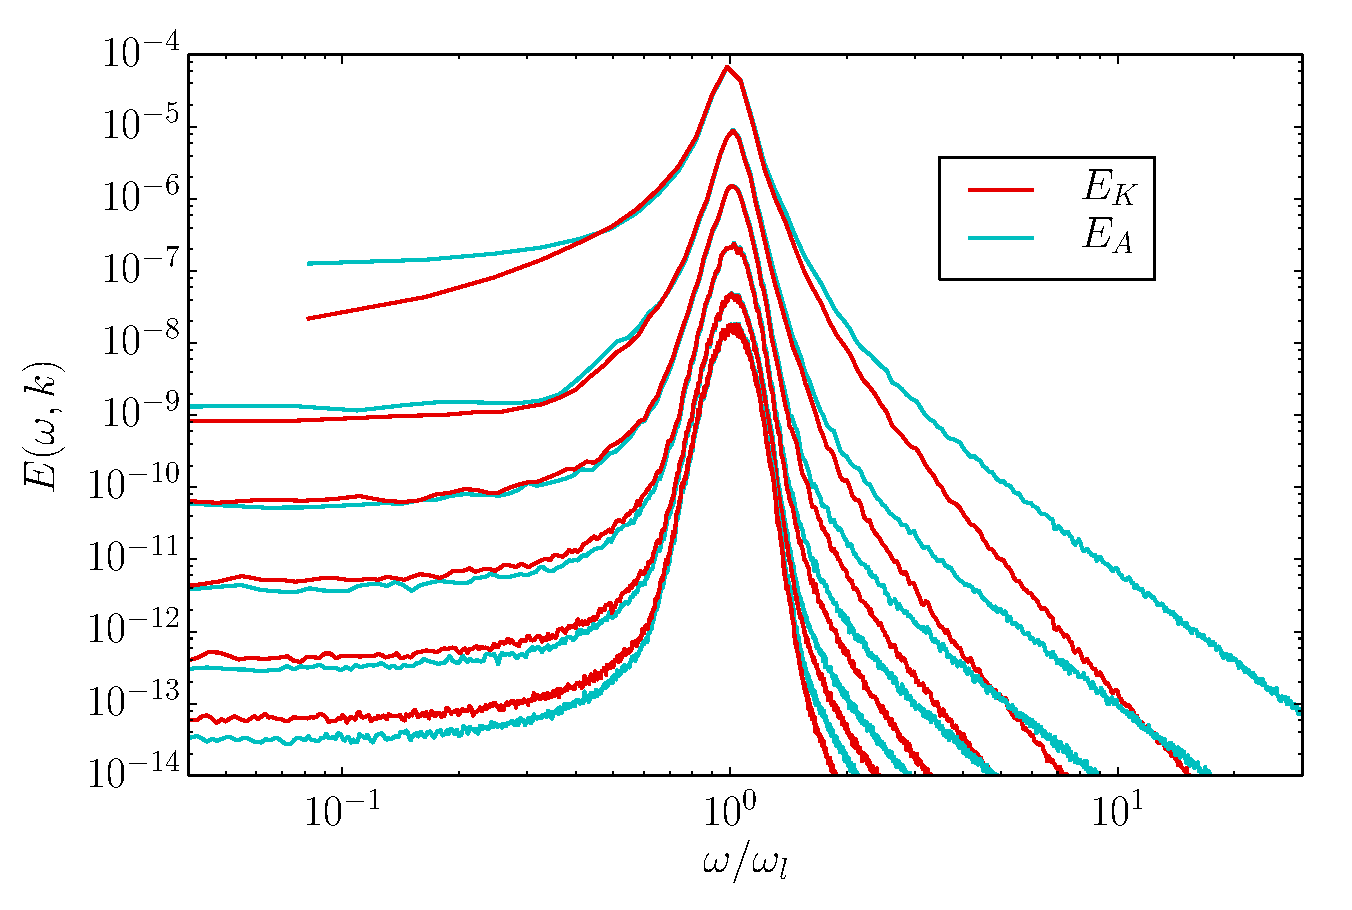
\includegraphics[width=3.15in]{../Old/Figs/fig_spatiotempspectra_c20_Nh3840}}
\caption{Spatio-temporal spectra of KE (dark lines) and APE (light
lines) for $c = 20$ and $n = 3840$ versus $\omega/\omega_l$, where
$\omega_l = c k$.  From the larger to the smaller spectra, $k/\delta k
= 12$, 27, 62, 143, 327, and 746.  }
\label{fig_spatiotemp_spectra}
\end{figure}

Figure~\ref{fig_spatiotemp_spectra} presents the spatio-temporal
spectra plotted as a function of the normalized frequency
$\omega/\omega_l$.
%\PA{Explain how these spectra have been calculated.}
In order to calculate these spectra, we have saved well-resolved time
series of $\hat d(\kk)$ and $\hat a(\kk)$ for wave numbers inside
particular shells such as $k\leqslant \kk<k+\delta k$, computed the
temporal spectrum of each signal and averaged over the wave numbers
inside each shell.
%
The spectra are strongly dominated by large peaks at $\omega =
\omega_l$ indicating that the characteristic frequency for each wave
number is the linear frequency.  However, the widening of the peaks
can be explained only by nonlinear effects.  \Add{The equipartition
between kinetic and potential energies is expected since the flow only
consists of gravity waves and the total energy is nearly equal to the
quadratic energy which is equal to the sum over all waves of their
equipartitioned quadratic energy.}












\subsection{Time- and space-averaged energy as a function of $c$}

\begin{figure}
\centerline{
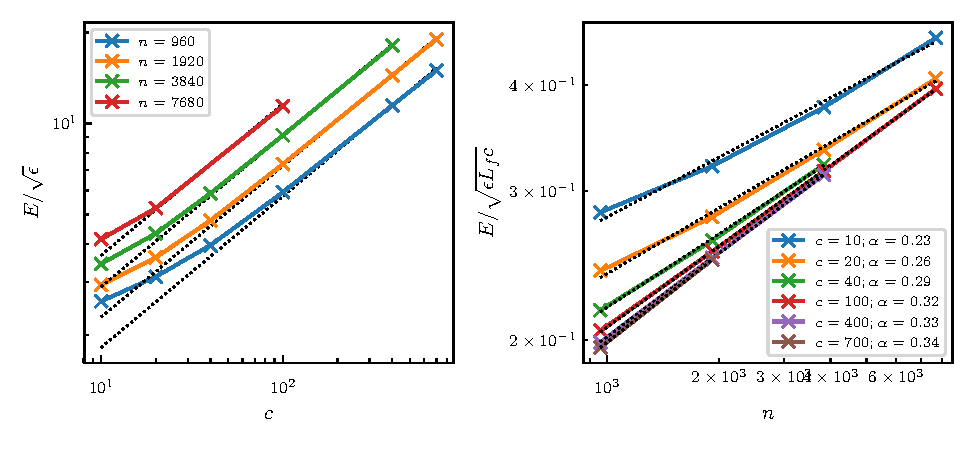
\includegraphics[width=\linewidth]{../Pyfig/fig_energy_w}
}
\caption{Time- and space-averaged energy
$\langle h|\uu|^2 + c^2 h^2 \rangle/2$
of the statistically stationary flows.
%
In (\textit{a}), the energy is divided by
$\sqrt{\eps}$ and plotted versus $c$ for 3 resolutions:
$n = 960$, dotted lines;
$n = 1920$, continuous lines and
$n = 3840$, dashed lines.
The cyan curves show the law $C_n \sqrt{\eps L_f c}$,
with $C_n$ a fit coefficient.
%
In (\textit{b}), the energy is divided by
$\sqrt{\eps L_f c}$ and plotted versus $n$
for six values of $c$ as indicated in the legend.
}
\label{fig_Evsc}
\end{figure}


Figure~\ref{fig_Evsc}(\textit{a}) shows the time- and space-averaged
energy for the statistically stationary flows divided by the square
root of the mean energy dissipation rate as a function of $c$ and for
three resolutions: $n = 960$, dotted lines; $n = 1920$, continuous
lines and $n = 3840$, dashed lines.
%
For all resolutions, the energy increases with $c$.  More precisely,
the curves can be well fitted to a law $E = C_n \sqrt{\eps L_f c}$
(blue lines).  However, the coefficient $C_n$ varies with the
resolution, i.e.\ with the effective Reynolds number.
%
This is very different from the case of isotropic turbulence where the
energy scales as $E \sim (\eps L_f)^{2/3}$ and does not vary with the
Reynolds number in the limit of very large Reynolds number.
%
Weak wave turbulence theory predicts an energy-flux law of the form $E
\propto \eps^{1/(N-1)}$, where $N$ is the number of waves involved
in the nonlinear interactions \cite[]{Nazarenko2011}.  Therefore, the
scaling $E = C_n \sqrt{\eps L_f c}$ would correspond to interactions
involving three waves.
%
However, the hypothesis needed for applying the weak wave turbulence
formulation are not fulfilled.


This effect of the increase of the energy with the resolution is
investigated in figure~\ref{fig_Evsc}(\textit{b}) where the quantity
$C_n = E/\sqrt{\eps L_f c}$ is plotted as a function of the
resolution.
%
For $c = 10$ (dotted line), the waves are not very fast and the
variation with the resolution is weak.
%
However, in the limit of very fast waves ($c>100$), the curves for the
different wave speeds nearly collapse and increase at least up to $n =
5760$.  The increase tends to saturate but it is difficult to know
from our results what is the scaling of $C_n$ as a function of the
resolution and if it really saturates for very large $n$ and $c$.
%
In order to decide on this issue, we would need to run simulations in
the very-fast-wave regime, $c>100$, and at very large resolutions $n >
5760$.  In this regime the energy fluctuations are large so
that the simulations would have to be carried out for very long time
in order to get a good convergence for the mean energy.  Since the
time step has to be extremely small in this regime, such simulations
would be too costly.





\subsection{Energy spectra}


We now turn to the study of the energy spectra.  A dimensional
analysis based on the assumption that the spectra only depend on
$\eps$, $c$ and $k_f$ gives the following general expression
\begin{equation}
E_{\alpha, \beta}(k) = k^{-\alpha} \eps^\beta   c^{2- 3\beta}
{k_f}^{\alpha -1 - \beta}, \label{eq_E_alpha_beta}
\end{equation}
where $\alpha$ and $\beta$ are two free parameters.



\begin{figure}
% \centerline{
% \includegraphics[width=\halfwidth]{../Figs/fig_spectra_c_Nx=1920_k32}
% \includegraphics[width=\halfwidth]{../Figs/fig_spectra_c_Nx=3840_k32}
% }
% \centerline{
% \includegraphics[width=\halfwidth]{../Figs/fig_spectra_c_Nx=1920_k2}
% \includegraphics[width=\halfwidth]{../Figs/fig_spectra_c_Nx=3840_k2}
% }
\caption{
Compensated energy spectra versus $k/k_f$ for different wave speeds $c$.
%
The spectra are compensated by $k^{-3/2}\sqrt{\varepsilon c} $
in (\textit{a,b})
and by $k^{-2}c^{1/3} \eps^{5/9} k_f^{4/9} $
in (\textit{c,d}).
%
The resolution is
$n = 1920$ in (\textit{a,c}) and
$n = 3840$ in (\textit{b,d}).
%
In (\textit{a,c}), the wave speed goes from 10 to 1000
and
in (\textit{b,d}) from 10 to 200
(for the precise values, see figure~\ref{fig_Evstime}).
}
\label{fig_spectra_c}
\end{figure}


The scaling of the energy as $\sqrt{\eps L_f c}$ suggests that the
spectra should scale like the Zakharov-Sagdeev spectrum, $E(k) \sim
k^{-3/2}\sqrt{\eps c}$, which is the prediction of weak wave
turbulence theory for three-dimensional acoustic turbulence
\cite[]{Nazarenko2011}.
%
The compensated spectra $E(k) / ( k^{-3/2}\sqrt{\eps c})$ are plotted
in figure~\ref{fig_spectra_c}(\textit{a}) for $n = 1920$ and in
figure~\ref{fig_spectra_c}(\textit{b}) for $n = 3840$.  The different
curves correspond to different wave speeds, going from $c=10$ to
$c=1000$ for $n = 1920$ and from $c=10$ to $c=200$ for $n = 3840$.
%
For both resolutions, the compensated spectra collapse at the
energy-dominating small wave numbers.
%
However, these compensated spectra are not flat in the inertial range
and do not collapse in the inertial and dissipation ranges, i.e. for
$k\gtrsim 2k_f$.  In the inertial range, they follow a clear $k^{-2}$
scaling law and there is a bottleneck in the dissipation range where
the slope is close to $-3/2$.
%
\cite{Kuznetsov2004} showed that $k^{-2}$ spectra can be explained by
singularities and this scaling has already been observed in
two-dimensional acoustic turbulence \cite[]{FalkovichMeyer1996}.
%

Inserting $\alpha = 2$ in the spectrum (\ref{eq_E_alpha_beta}) gives
\begin{equation}
E_\beta(k) = k^{-2} {k_f}^{1-\beta} c^{2-3\beta} \eps^\beta
\end{equation}
and we have found that the numerical spectra are very close to the
spectrum $E_\beta(k)$ with $\beta = 5/9$.
%
The compensated spectra $E(k) / ( k^{-2} c^{1/3} \eps^{5/9} k_f^{4/9}
)$ are plotted in figure~\ref{fig_spectra_c}(\textit{c}) for $n =
1920$ and in figure~\ref{fig_spectra_c}(\textit{d}) for $n = 3840$.
The collapse is very good in the inertial range but we stress that we
are not aware of any theory predicting the empirical spectrum $k^{-2}
c^{1/3} \eps^{5/9} k_f^{4/9}$.





\begin{figure}
\centerline{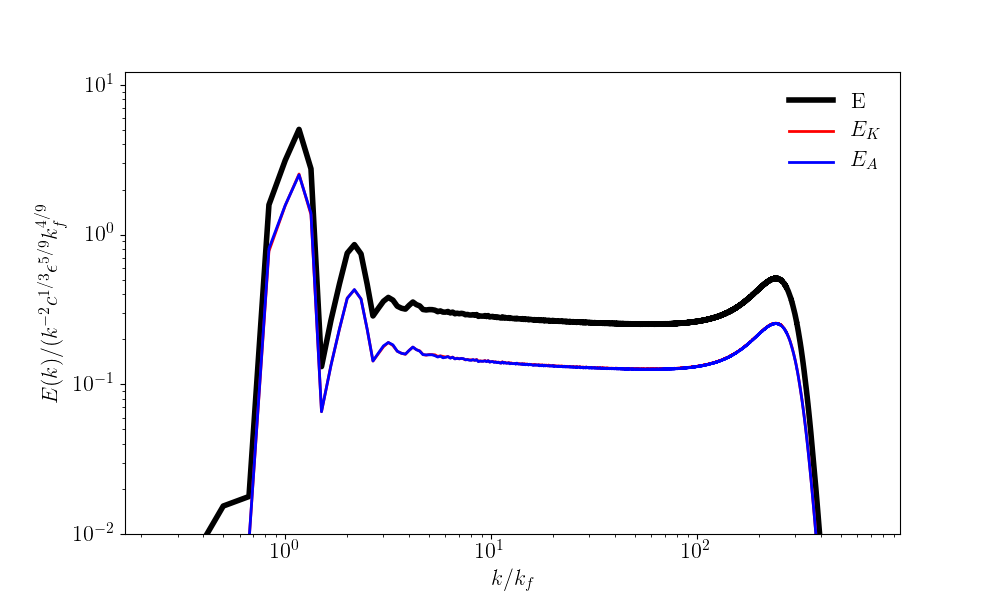
\includegraphics[width=8cm]{../Pyfig/fig_spectra_c=100_nh=7680}}
\caption{Compensated spectra
of total energy (thick black line)
kinetic energy (thin dark line) and
available potential energy (thin light line)
for $c = 40$ and $n = 7680$.}
\label{fig_spectra_c40}
\end{figure}

Figure~\ref{fig_spectra_c40} shows the compensated spectra $E(k) / (
k^{-2} c^{1/3} \eps^{5/9} k_f^{4/9} )$ of total energy (black line),
KE (red line) and APE (blue line) for $c = 40$ and $n = 7680$.  For
all wave numbers, we have $E(k) = 2E_K(k) = 2E_A(k)$ since the flow
only consists of \Add{gravity} waves.
%
The spectra are very close to $k^{-2}$ in the inertial range over more
than one decade and the shallowing to a slope close to $-3/2$ is
clearly confined to the dissipation range.  This confirms that this
bump is due to a dissipation effect and that there is no wide
$k^{-3/2}$ spectrum even at very large resolutions.


% \begin{figure}
% \centerline{
% \includegraphics[width=\halfwidth]{../Figs/fig_spectra_resol_c=10}
% \includegraphics[width=\halfwidth]{../Figs/fig_spectra_resol_c=40}
% }
% \caption{Compensated energy spectra $E(k) / ( k^{-3/2}\sqrt{\eps c})$
% for different resolutions.  In (\textit{a}), $c = 10$ and in
% (\textit{a}), $c = 40$.}
% \label{fig_spectra_resol}
% \end{figure}

% The compensated spectra $E(k) / ( k^{-3/2}\sqrt{\eps c})$ are plotted
% for different resolutions %
% in figure~\ref{fig_spectra_resol}(\textit{a}) for $c=10$ and
% in figure~\ref{fig_spectra_resol}(\textit{b}) for $c=40$.
% %
% We see that an inertial range with a $k^{-2}$ scaling starts to appear
% for $n\gtrsim 960$.
% %
% As seen in figure~\ref{fig_Evsc}, the ratio $E/\sqrt{\eps L_f c}$ only
% weakly varies for $c=10$ but increases in the fast-waves regime for
% $c=40$.  This effect can be seen here at the energy-containing wave
% numbers $k<2 k_f$.  However, the variation with the resolution is much
% weaker in the inertial range at $k>2 k_f$.



In subsection~\ref{subsection_cascade}, we have shown that third-order
structure functions scale like $r$ since there is a downscale energy
cascade.
%
The Kolmogorov method predicts $k^{-5/3}$-spectra but the numerical
spectra are much steeper in the inertial range, with a slope equal to
-2.  The fact that third-order and second-order quantities can not be
simply related by the Kolmogorov scaling implies that the cascade is
very intermittent.




\subsection{Effect of the shocks and intermittency}




\begin{figure}
% \setlength{\halfwidth}{2.72in}
\centerline{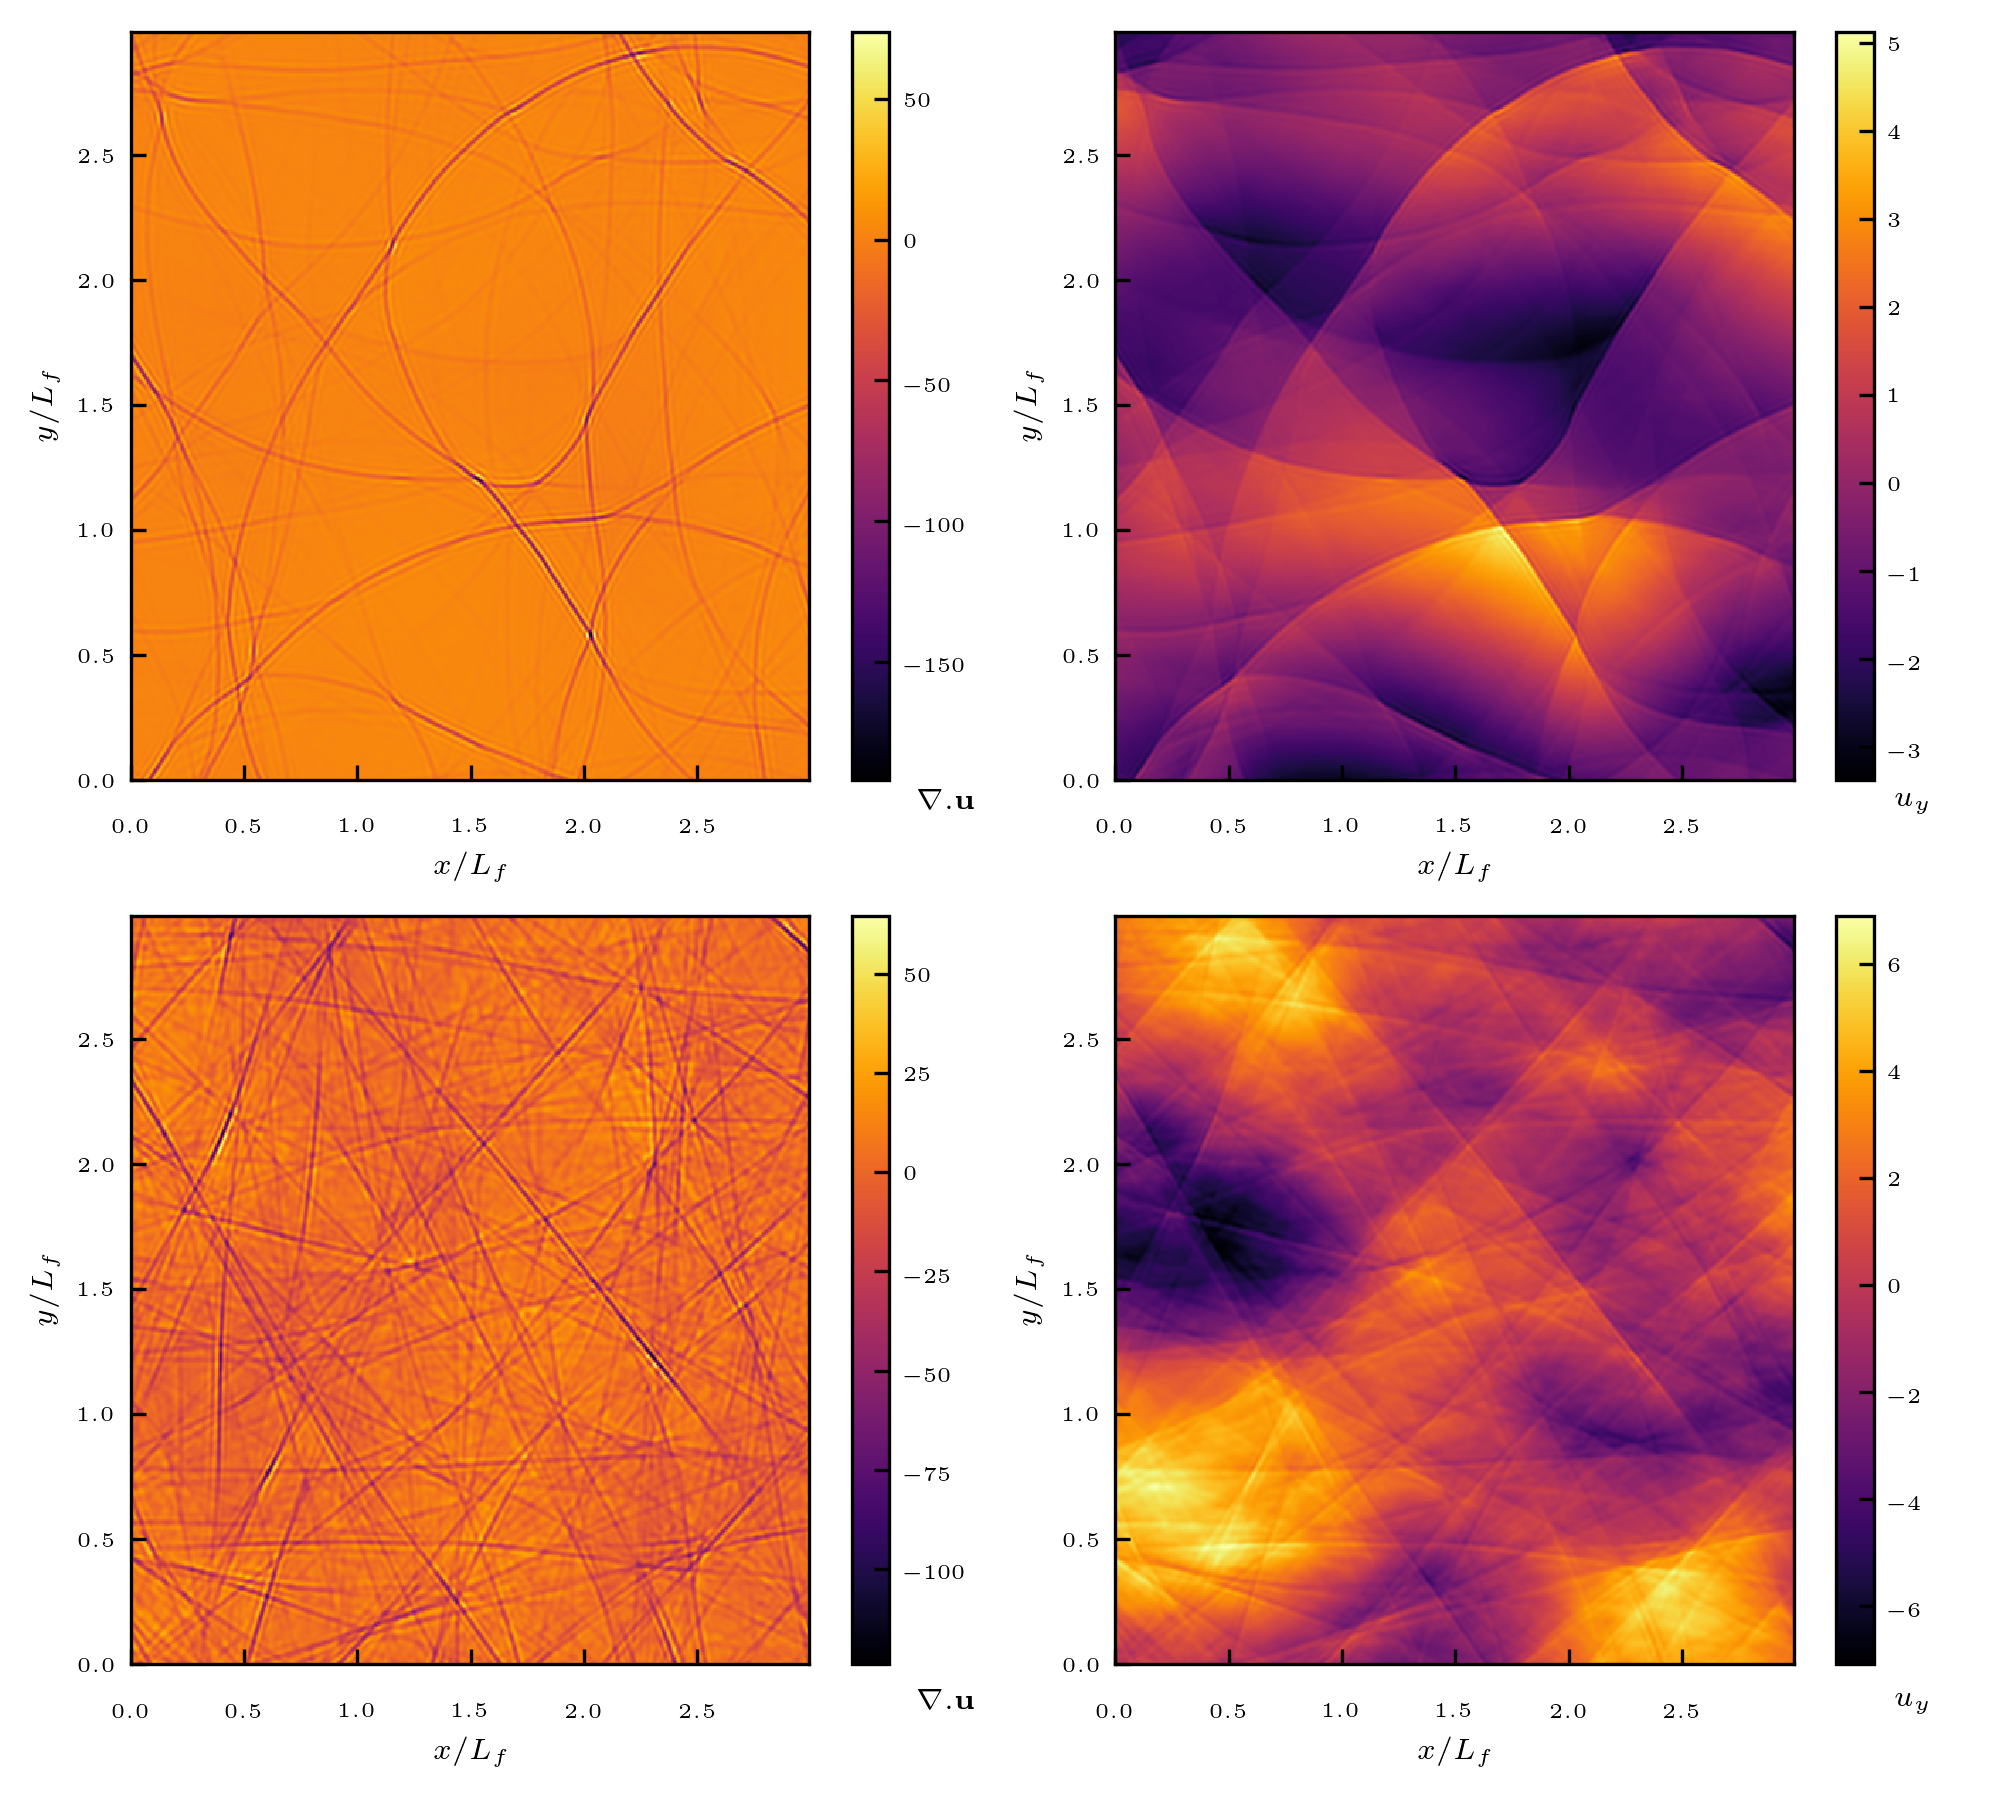
\includegraphics[width=5.20in]{../Pyfig/fig_phys_fields_wave}}
% \centerline{
% \includegraphics[width=\halfwidth]{../Figs/fig_2Dh_c20}
% \hspace{-4mm}
% \includegraphics[width=\halfwidth]{../Figs/fig_2Dh_c200}
% }
% \centerline{
% \includegraphics[width=\halfwidth]{../Figs/fig_2Duy_c20}
% \hspace{-4mm}
% \includegraphics[width=\halfwidth]{../Figs/fig_2Duy_c200}
% }
\caption{
Snapshots for $n = 1920$ and two values of the wave speed
$c= 20$ (\textit{a,c}) and $c= 200$ (\textit{b,d}).
The colors represent the thickness in (\textit{a,b}) and
the $y$-component of the velocity in (\textit{c,d}).
The arrows represent the velocity field.
%
The coordinates are nondimensionalized by the characteristic scale of
the forcing $L_f = 3.57$.  }
\label{fig_phys}
\end{figure}

Figure~\ref{fig_phys} shows %
the normalized thickness $h$ %
(figures~\ref{fig_phys}\textit{a,b}) %
and the $y$-component of the velocity $u_y$ %
(figures~\ref{fig_phys}\textit{c,d}) %
for $c = 20$ (figures~\ref{fig_phys}\textit{a,c}) and %
$c = 200$ (figures~\ref{fig_phys}\textit{b,d}).
%
These wave speeds correspond %
to a moderate forcing Froude number $F_f \sim 0.05$ and %
to a very small forcing Froude number $F_f \sim 0.005$, respectively.
The normalized surface displacement $\eta = h - 1$ is of order 0.3 for
$c = 20$ and one order of magnitude smaller, 0.03, for $c = 200$.
%
The typical velocity is also much smaller than the wave speed, %
with $u_y/c \sim 0.2$ for $c = 20$ %
and $u_y/c \sim 0.03$ for $c = 200$. %
This confirms that the flows are in a fast-wave regime, especially for
$c = 200$.
%
However, many discontinuities can be seen in both fields $h$ and
$u_y$.  These discontinuities are hydraulic jumps, which are the
equivalent to shocks in a compressible flows.
%
\Add{Baines (1998) provides a theoretical prediction for the velocity
of the hydraulic jumps is one-layer shallow-water flow:
\begin{equation}
c_s = c \sqrt{\frac{h_+}{h_-} \frac{h_+ + h_-}{2}},
\end{equation}
where $h_+$ and $h_-$ are the dimensionless thickness before and after
the jump.
%
We have verified that the velocity of the discontinuities in the
simulations is consistent with this theoretical prediction, implying
that the associated Froude number (or Mach number) is of the order
unity.}

\nocite{Baines1998}

% We have verified that these shocks are very fast and travel at a
% velocity of the order of the wave speed \Add{(more precisely, Baines 1998)}
% , implying
% that their associated Froude number (or Mach number) is of the order
% unity.
%el (This is not necessarily true...)
% The existence of shocks implies that there is a strong coherence
% between small and large wave numbers and indicates nonlocal
% interactions between wave numbers.
%
In between the shocks, the flow is very smooth for $c=20$ and slightly
more irregular for $c = 200$.

Figures~\ref{fig_phys}(\textit{c,d}) display the $y$-component of the
velocity.  There are less discontinuities in this quantity than in the
thickness. More precisely, the $h$-discontinuity lines that are along
the $y$-axis are not associated with corresponding discontinuities of
the $y$-component of the velocity. This can be seen for example for
the shock at $x/L_f\simeq 0.4$ and $y/L_f\simeq 2.1$ in
figures~\ref{fig_phys}(\textit{a}) and \ref{fig_phys}(\textit{c}).
%
This illustrates that the singularity in the velocity is in the
component perpendicular to the shock line, which is the assumption on
the structure of the velocity discontinuities used in the model
presented in \S~\ref{subsection_shock_model}.







\begin{figure}
% \centerline{
% \includegraphics[width=\halfwidth]{../Figs/fig_interm_strfct_ux}
% \includegraphics[width=\halfwidth]{../Figs/fig_interm_strfct_uy}
% }
\caption{
Compensated fifth-order structure functions $\mean{|\delta u_L|^5}/r$
of (\textit{a}) the longitudinal increments and (\textit{b}) the
transverse increments. %
The crosses indicate the range of separation $r$ where the exponent
$\zeta_p$ is computed. %
The dashed lines correspond to the Kolmogorov scaling laws $r^{p/3}$
and $\zeta_p = p/3$.  The wave speed and the resolution are $c = 40$
and $n = 7680$.  }
\label{fig_strfct5}
\end{figure}


The shock model derived in subsection~\ref{subsection_shock_model}
predicts that structure functions of all orders should scale linearly
with $r$.
%
Figure~\ref{fig_strfct5} presents fifth-order structure functions
compensated by $r$.
%
Figures~\ref{fig_strfct5}(\textit{a}) and
\ref{fig_strfct5}(\textit{b}) correspond to the structure functions
computed from the longitudinal increments and the transverse
increments, respectively.  The structure functions compensated by $r$
are nearly flat between $r \simeq 0.012 L_f$ and $r \simeq 0.06 L_f$,
showing that they scale like $r$ on this relatively narrow range of
scale compared to the inertial range.
%
The $r$-scaling is very different from the slope of the fifth-order
structure functions calculated from the Kolmogorov scaling $\zeta_5 =
p/3 \simeq 1.66$ (dashed straight line).  This shows that the wave
cascade is strongly intermittent and that this intermittency can be
explained by the presence of discontinuities related to the shocks.




\begin{figure}
% \centerline{
% \includegraphics[width=\halfwidth]{../Figs/fig_interm_ux}
% \includegraphics[width=\halfwidth]{../Figs/fig_interm_uy}
% }
\caption{
Exponents $\zeta_p$ of the structure functions
of (\textit{a}) the longitudinal increments
and (\textit{b}) the transverse increments versus the order $p$.
%
The dashed lines correspond to
the Kolmogorov scaling laws $r^{p/3}$ and $\zeta_p = p/3$.
The wave speed and the resolution are $c = 40$ and $n = 7680$.
}
\label{fig_interm}
\end{figure}






The slope of the structure functions of order $p$ over the range
$0.012 L_f\leqslant r \leqslant 0.06 L_f$, $\zeta_p$, are plotted in
figure~\ref{fig_interm}(\textit{a}) for the longitudinal increments
and in figure~\ref{fig_interm}(\textit{b}) for the transverse
increments.
%
The exponent are very far from the Kolmogorov scaling $\zeta_p = p/3$.
They increase as $p$ for $p\ll1$, saturate to a value close to 1 for
$p>2$ and tend to decrease for $p>3$.
%
A similar shape of the $\zeta_p$ function has been predicted for
Burger turbulence \cite[]{BouchaudMezardParisi1995}.
%
The shape of $\zeta_p$ at very small $p$ is determined by the
scaling of the smallest velocity increments and the $p^1$-variation
shows that these smallest increments scales like $\delta u \sim r^p$.
%
The plateau at $p > 2$ is a consequence of the dominance by shocks of
the largest increments.
%
Note that these results are obtained for a relatively small forcing
Froude number $F_f \simeq 0.03$ corresponding to $c=40$.  The function
$\zeta_p$ has approximately the same extreme shape for a larger Froude
number $F_f \simeq 0.01$, corresponding to $c=10$.  Note also that the
decrease of $\zeta_p$ for $p>3$ is anomalous, which could be due to
the relatively narrow width of the range over which $\zeta_p$ is
computed.



\begin{figure}
\centerline{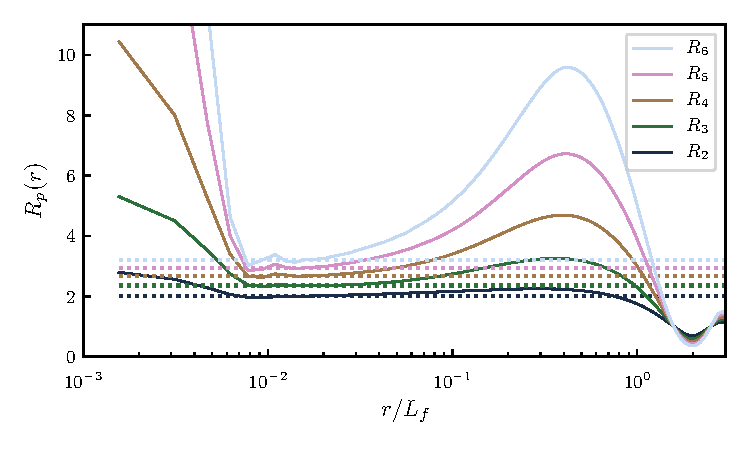
\includegraphics[width=\halfwidth]{../Pyfig/fig_ratio_strfct}}
\caption{
Ratio of the structure functions of the velocity increments
$R_p(r) \equiv \mean{|\delta u_L|^p} / \mean{|\delta u_T|^p}$
for $p = 2,$ 3 and 4.
The dotted straight lines indicate the values computed by the shock model:
$R_2 = 2$, $R_3 = 6\pi/8$ and $R_4 = 8/3$.
%
The wave speed and the resolution are $c = 10$ and $n = 7680$.  }
\label{fig_ratio}
\end{figure}


The functions $R_p = \mean{|\delta u_L|^p}/\mean{|\delta u_T|^p}$ are
plotted in figure~\ref{fig_ratio} for $p =2$ to 4.  The predictions of
the shock model, $R_2 = 2$, $R_3 = 6\pi/8$ and $R_4 = 8/3$, are also
plotted in dotted lines for comparison.  We see that the numerical
results are reasonably close to these predictions.  However, the
agreement is less good for smaller Froude number (not shown).  The
structure functions are fully determined by shocks only for Froude
numbers that are not too small, which is consistent with the snapshots
in figure~\ref{fig_phys} showing that the fields between the shocks
are more irregular for the smallest Froude number.


\begin{figure}
\centerline{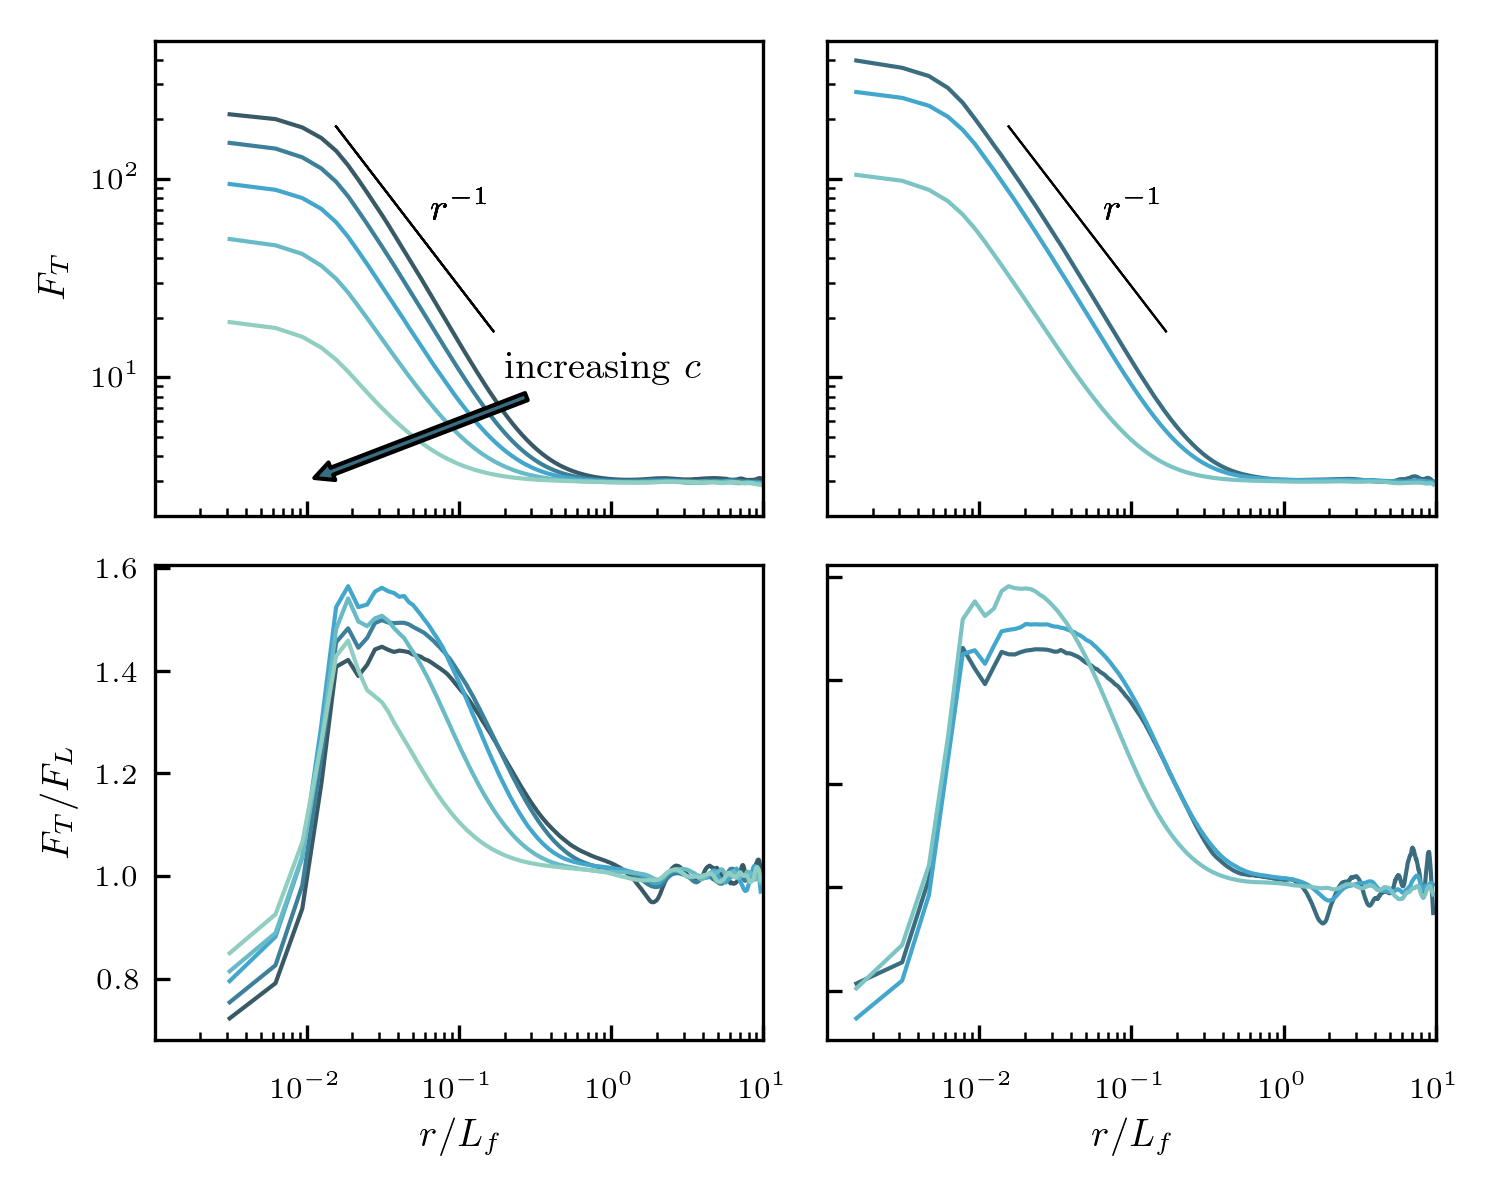
\includegraphics[width=5.12in]{../Pyfig/fig_flatness}}
\caption{ Flatness of the longitudinal and transverse increments for
$c = 10$ and $n = 7680$. The straight continuous lines indicate the
$r^{-1}$-scaling and the straight dashed line the $r^{-3/2}$-scaling.
The inset shows the ratio $F_T/F_L$ and the corresponding value
computed by the shock model, $F_T/F_L = 1.5$.  }
\label{fig_flatness}
\end{figure}
%
Figure~\ref{fig_flatness} shows the flatness of the longitudinal and
transverse increments, computed from a numerical simulation for $c =
10$ and $n = 7680$.
%
For a Gaussian probability distribution the flatness factor is equal
to 3 whereas the shock model predict flatness factors scaling like
$r^{-1}$.
%
We see that here the flatness factors are much larger than 3, of the
order of $10^3$.
%
Remarkably, they scale approximately as $r^{-1}$ as predicted by the
shock model and the ratio $F_T/F_L$ is very close to the predicted
value 1.5.



% Figure~\ref{fig_flatness}(\textit{b}) shows the same quantities
% computed from atmospheric data measured by commercial aircraft.
% %
% The flatness curves have been taken from \cite{Lindborg1999}.
% Surprisingly, the atmospheric results are quite similar to the
% numerical ones. The flatness factors are very large and strongly
% decrease at scales smaller than 100 km.  Interestingly, the ratio
% $F_T/F_L$ is also very close to the value 1.5 predicted by the shock
% model.
% %
% We stress that even though these similarities are striking, the
% underlying dynamics are very different.
% %
% While there is no energy in the quasi-geostrophic modes in the
% numerical simulations, the atmospheric flows are usually close to be
% quasi-geostrophic at horizontal scales larger than 500 km and the
% vertical vorticity is in average of the same order of magnitude than
% the horizontal divergence at the mesoscales, i.e. at horizontal scales
% between 10 and 500 km \cite[]{Lindborg2007jas}.
% %
% Therefore, it is not surprising to also see differences between the
% atmospheric and the numerical results. The flatness factors in
% figure~\ref{fig_flatness}(\textit{b}) vary approximately as $r^{-3/2}$
% (dashed line), which is significantly faster than for the numerical
% simulations of the shallow-water model. Moreover, the second-order
% structure functions in the atmosphere scale as $r^{2/3}$
% \cite[]{Lindborg1999, ChoLindborg2001,
% FrehlichSharman2010}. Considering the scaling for the flatness
% factors, this implies that the variation with scale of the
% fourth-order structure functions is actually very weak, which is
% not in agreement with the prediction of the shock model.
% %
% Nevertheless, we do not know other explanations of such very large
% flatness factors with a ratio $F_T/F_L=1.5$ observed in the atmosphere.
% %
% Thus, we think that these results raise interesting questions
% regarding the interpretation of structure functions measured in the
% atmosphere.  How important are the discontinuities on horizontal
% cross-sections in these cases?
% %
% It is well known that the fronts separating cold and warm regions
% explain many meteorological phenomena.
% %
% The curves in figure~\ref{fig_flatness} seem to indicate that
% they could also have strong effects on the statistics of the atmosphere
% over a quite large range of scales.
